\documentclass{article}
\usepackage[preprint]{neurips_2026}
\usepackage[utf8]{inputenc}
\usepackage[T1]{fontenc}
\usepackage[spanish,es-tabla]{babel}
\usepackage{amsmath,amssymb,booktabs,graphicx,microtype,url}
\usepackage{hyperref}
\newcommand{\pending}[1]{\paragraph{Pendiente de evidencia.} #1}
\author{Grupo de cinco estudiantes: completar nombres y correos\\
Universidad Nacional de Ingeniería\\Lima, Perú}

\usepackage{float}
\title{Segmentación de agua en Sentinel-1: U-Net propia, supervisión débil y generalización a Bolivia}
\begin{document}
\maketitle
\begin{abstract}
Se compara una U-Net implementada directamente en PyTorch sobre los canales VV/VH de
Sen1Floods11. El protocolo cruza etiquetas manuales y manuales más débiles con las pérdidas
BCE, Dice y su suma; conserva la validación manual y reserva Bolivia exclusivamente para
evaluación externa. La auditoría verifica 9\,216 archivos y excluye 16 chips sin píxeles válidos.
Se reportan IoU promedio por chip, métricas agrupadas por píxel y una convención adicional
compatible con el tratamiento de unión vacía de la referencia oficial.
\InputIfFileExists{abstract_results.tex}{}{Los resultados científicos se incorporan al terminar las seis configuraciones.}
\end{abstract}

\section{Problema y trabajos relacionados}
El objetivo es asignar una probabilidad de agua a cada píxel válido de una observación SAR.
Las observaciones de radar permiten estudiar eventos bajo nubosidad, pero su interpretación
depende de geometría, rugosidad y propiedades dieléctricas de la superficie~\cite{sarhandbook}.
La clase positiva de Sen1Floods11 incluye agua observada y no diferencia por sí sola
inundación nueva de agua permanente~\cite{sen1}. Por ello, este trabajo evalúa segmentación
de agua y no estima daño, profundidad ni extensión temporal de inundación.

U-Net combina un encoder contextual con conexiones de salto que conservan detalle
espacial~\cite{unet}. Se implementan sus bloques sin descargar una arquitectura o pesos
preentrenados. Dice permite optimizar solapamiento~\cite{vnet}; aquí se utiliza una variante
bidimensional con sumas de probabilidades, distinta del denominador cuadrático de V-Net.
La supervisión débil aumenta cobertura, pero puede introducir errores sistemáticos de
etiquetado~\cite{snorkel}. AdamW separa adaptación y decaimiento de pesos~\cite{adamw}.
GroupNorm calcula estadísticas por grupos de canales y resulta independiente del tamaño
del batch~\cite{groupnorm}. Estas decisiones permiten estudiar fuente de supervisión y
pérdida manteniendo constante el modelo.

\section{Datos y auditoría reproducible}
Se utiliza v1.1, con chips GeoTIFF de $512\times512$ píxeles, dos bandas VV/VH en dB y
etiquetas manuales o débiles de Sentinel-1. Se conservan los CSV oficiales de entrenamiento,
validación, prueba y Bolivia. Los 446 chips manuales se reparten originalmente en
252/89/90/15; nunca se incorporan todos al entrenamiento.

Los originales locales contienen 4\,160 pares débiles fuera de Bolivia. El inventario
remoto consultado el 3 de octubre de 2026 contiene 4\,384 pares, de los cuales 224 son de
Bolivia; la documentación menciona 4\,385. Se registra esa discrepancia de una unidad y no
se supone que un archivo inexistente deba descargarse. Los 4\,160 pares admisibles coinciden
con los nombres y tamaños del inventario remoto. No hay solapamientos con identificadores
manuales. La verificación local de tamaño y MD5 de los 9\,216 archivos seleccionados pasó
sin fallos; las huellas SHA-256 de imágenes, etiquetas y CSV quedan en el manifiesto.

Se comprueba correspondencia imagen/máscara, dos bandas SAR, una banda de etiqueta,
dimensiones, CRS y transformación afín. Se acepta únicamente redondeo numérico absoluto
menor o igual a $10^{-12}$ en sus coeficientes; no se remuestrea ninguna máscara. Los valores
válidos son 0 y 1. Se excluyen -1, nodata del raster e intensidades no finitas en cualquiera
de las dos bandas. La auditoría encontró 16 chips totalmente inválidos: uno de entrenamiento,
tres de validación, dos de prueba y diez débiles; ninguno de Bolivia. Los IDs excluidos
quedan persistidos para poder reproducir los conteos efectivos.
\begin{table}[H]\centering\small
\caption{Inventario efectivo después de excluir nodata.}
\begin{tabular}{lrrr}
\toprule
Partición & Chips & Píxeles válidos & Fracción agua \\
\midrule
train & 251 & 57017597 & 0.0955 \\
val & 86 & 20274154 & 0.1101 \\
test & 88 & 20443959 & 0.1230 \\
bolivia & 15 & 2824434 & 0.1600 \\
weak & 4150 & 1069346608 & 0.1683 \\
\bottomrule
\end{tabular}
\end{table}


Las estadísticas se calculan únicamente sobre píxeles válidos del entrenamiento manual,
después de recortar intensidades al intervalo fijo $[-50,10]$ dB. Las medias VV/VH son
$-10.4551/-17.3253$ dB y las desviaciones $4.0661/4.7918$ dB. Se aplican las mismas
estadísticas a todas las fuentes y particiones. El clipping limita valores extremos, pero
puede saturar señales informativas. En el tensor de entrada, los píxeles inválidos se
reemplazan por cero normalizado; siguen excluidos de pérdidas y métricas.
La proporción positiva válida es 9.55\% en entrenamiento y 16.00\% en Bolivia.
Esta diferencia de prevalencia puede afectar precisión y métricas agregadas.

Los originales se montan en solo lectura. Una caché independiente en un volumen Linux
se copia y vuelve a verificar contra MD5 para evitar el coste de acceso repetido desde
Windows. Contiene los mismos archivos, sin convertir valores, modificar geometría ni
agregar observaciones. Sentinel-2 queda fuera del alcance de este experimento.

\section{U-Net personalizada}
La entrada tiene forma $B\times2\times H\times W$ y la salida un logit por píxel.
Cada bloque contiene dos convoluciones $3\times3$ sin sesgo, GroupNorm de ocho grupos
y ReLU. El encoder usa 32, 64, 128 y 256 canales, con max-pooling $2\times2$;
el bottleneck tiene 512. Cada etapa del decoder aplica convolución transpuesta
$2\times2$, concatena el salto del encoder y refina con otro bloque. Una convolución
$1\times1$ produce la salida. Se interpola a la dimensión del salto si las formas
difieren, comportamiento verificado también para tamaños impares. Las imágenes reales
mantienen su resolución de $512\times512$. El modelo tiene 7\,762\,753 parámetros.

La arquitectura se inicializa desde cero. GroupNorm evita estimar estadísticas a partir de
cuatro ejemplos; no elimina los otros efectos del batch sobre la optimización. Las
aumentaciones son flips horizontales y verticales sincronizados entre bandas y máscara,
con probabilidad 0.5 por eje. No se inventan intensidades ópticas ni se rotan canales.

\section{Pérdidas y confianza de supervisión}
Para el conjunto de píxeles válidos $V_k$ del chip $k$ y $p_i=\sigma(z_i)$:
\begin{equation}
\mathcal{L}_{BCE,k}=-\frac{1}{|V_k|}\sum_{i\in V_k}
\left[y_i\log p_i+(1-y_i)\log(1-p_i)\right].
\end{equation}
Se evalúa de forma estable directamente sobre logits. La variante Dice es
\begin{equation}
\mathcal{L}_{Dice,k}=1-\frac{2\sum_{i\in V_k}p_i y_i+\epsilon}
{\sum_{i\in V_k}p_i+\sum_{i\in V_k}y_i+\epsilon},\qquad\epsilon=10^{-6}.
\end{equation}
La pérdida combinada suma ambos términos sin un coeficiente adicional. Para $K$ chips
válidos del batch se optimiza $K^{-1}\sum_k w_k\mathcal{L}_k$, con $w_k=1$ para
etiquetas manuales y $w_k=0.3$ para débiles. Dividir por $K$, en vez de por la suma de
pesos, conserva la atenuación 0.3 incluso en batches enteramente débiles.
Las reducciones se calculan en FP32 dentro del entrenamiento con precisión mixta.

Cada chip aporta un término antes del promedio, independientemente del número de píxeles
válidos; no se confunde esta ponderación con un promedio global por píxel. No se balancea
el número de chips por fuente. En la condición mixta, 4\,150 débiles y 251 manuales implican
que 83.2\% de la masa nominal de pesos corresponde a supervisión débil. Ese cálculo
describe el muestreo, no la contribución efectiva de cada gradiente.

\section{Diseño experimental y evaluación}
Se ejecutan seis configuraciones con semilla 42: \texttt{gold} y \texttt{gold\_weak},
cada una con BCE, Dice y su suma. Los parámetros comunes son batch 4, AdamW,
tasa $3\times10^{-4}$, decaimiento $10^{-4}$, clipping de norma de gradiente a 1,
hasta 50 épocas y paciencia 10 sobre pérdida de validación manual. Se restaura el
checkpoint de mínima pérdida de validación de cada corrida. El umbral 0.5 se fija antes
de evaluar y Bolivia no participa en normalización, entrenamiento o selección.
La ejecución habilita semillas y algoritmos deterministas con avisos; no se afirma
identidad numérica garantizada entre hardware o versiones diferentes.

La comparación controla arquitectura e hiperparámetros, pero no presupuesto de actualizaciones:
una época manual tiene 63 pasos y una mixta 1\,101. La supervisión y el número de pasos
cambian conjuntamente. Además, las escalas BCE/Dice/combinada difieren; no se comparan sus
valores absolutos de pérdida como medida de calidad entre configuraciones.

La métrica principal es el promedio no ponderado de IoU por chip con unión no vacía:
$\mathrm{IoU}_k=TP_k/(TP_k+FP_k+FN_k)$. Una unión vacía es indefinida y se informa
como tal, con el número de chips excluidos. Se presenta también
$(TP_k+10^{-7})/(TP_k+FP_k+FN_k+10^{-7})$, que asigna uno a la unión vacía,
siguiendo el tratamiento del notebook oficial; esto no convierte todo el protocolo en
una réplica de su modelo. Ambas convenciones se mantienen visibles.

Para los conteos acumulados en píxeles válidos se reportan IoU, precisión
$TP/(TP+FP)$, recall $TP/(TP+FN)$, F1, omisión $1-\mathrm{recall}$ y comisión
$1-\mathrm{precision}$. Un denominador nulo queda como no definido. La IoU global
pondera indirectamente chips por área de unión, por lo que no equivale al promedio por chip.
La brecha geográfica es $\mathrm{IoU}_{ID}-\mathrm{IoU}_{Bolivia}$; puede ser negativa.
Se evalúan los 88 chips ID y 15 de Bolivia para cada configuración.

\section{Resultados}
\begin{table}[H]\centering\small
\caption{IoU promedio sobre chips con unión no vacía. Brecha: ID menos Bolivia.}
\begin{tabular}{lrrr}
\toprule
Experimento & IoU ID & IoU Bolivia & Brecha \\
\midrule
gold\_bce & 0.3939 & 0.4555 & -0.0616 \\
gold\_dice & 0.4100 & 0.4463 & -0.0364 \\
gold\_combined & 0.4068 & 0.4057 & 0.0010 \\
gold\_weak\_bce & 0.3251 & 0.2690 & 0.0560 \\
gold\_weak\_dice & 0.3487 & 0.4790 & -0.1302 \\
gold\_weak\_combined & 0.3593 & 0.4511 & -0.0918 \\
\bottomrule
\end{tabular}
\end{table}
\begin{table}[H]\centering\small
\caption{Métricas agrupadas por píxel en prueba en distribución.}
\begin{tabular}{lrrrrrr}
\toprule
Experimento & IoU global & F1 & Prec. & Recall & Omisión & Comisión \\
\midrule
gold\_bce & 0.6642 & 0.7982 & 0.8538 & 0.7495 & 0.2505 & 0.1462 \\
gold\_dice & 0.6473 & 0.7859 & 0.7810 & 0.7908 & 0.2092 & 0.2190 \\
gold\_combined & 0.6611 & 0.7960 & 0.8256 & 0.7684 & 0.2316 & 0.1744 \\
gold\_weak\_bce & 0.6099 & 0.7577 & 0.7955 & 0.7233 & 0.2767 & 0.2045 \\
gold\_weak\_dice & 0.5902 & 0.7423 & 0.7262 & 0.7591 & 0.2409 & 0.2738 \\
gold\_weak\_combined & 0.6102 & 0.7579 & 0.7464 & 0.7698 & 0.2302 & 0.2536 \\
\bottomrule
\end{tabular}
\end{table}
\begin{table}[H]\centering\small
\caption{Métricas agrupadas por píxel en Bolivia.}
\begin{tabular}{lrrrrrr}
\toprule
Experimento & IoU global & F1 & Prec. & Recall & Omisión & Comisión \\
\midrule
gold\_bce & 0.6779 & 0.8081 & 0.8573 & 0.7642 & 0.2358 & 0.1427 \\
gold\_dice & 0.6385 & 0.7794 & 0.8104 & 0.7507 & 0.2493 & 0.1896 \\
gold\_combined & 0.5844 & 0.7377 & 0.8372 & 0.6593 & 0.3407 & 0.1628 \\
gold\_weak\_bce & 0.4807 & 0.6493 & 0.9185 & 0.5021 & 0.4979 & 0.0815 \\
gold\_weak\_dice & 0.7183 & 0.8361 & 0.8295 & 0.8428 & 0.1572 & 0.1705 \\
gold\_weak\_combined & 0.6942 & 0.8195 & 0.8826 & 0.7647 & 0.2353 & 0.1174 \\
\bottomrule
\end{tabular}
\end{table}
\begin{table}[H]\centering\small
\caption{Compatibilidad con la referencia oficial: epsilon de $10^{-7}$ y unión vacía igual a uno.}
\begin{tabular}{lrrrr}
\toprule
Experimento & Partición & Definidos & Unión vacía & IoU referencia \\
\midrule
gold\_bce & test & 86 & 2 & 0.4077 \\
gold\_bce & bolivia & 15 & 0 & 0.4555 \\
gold\_dice & test & 88 & 0 & 0.4100 \\
gold\_dice & bolivia & 15 & 0 & 0.4463 \\
gold\_combined & test & 88 & 0 & 0.4068 \\
gold\_combined & bolivia & 15 & 0 & 0.4057 \\
gold\_weak\_bce & test & 84 & 4 & 0.3557 \\
gold\_weak\_bce & bolivia & 15 & 0 & 0.2690 \\
gold\_weak\_dice & test & 87 & 1 & 0.3561 \\
gold\_weak\_dice & bolivia & 15 & 0 & 0.4790 \\
gold\_weak\_combined & test & 86 & 2 & 0.3739 \\
gold\_weak\_combined & bolivia & 15 & 0 & 0.4511 \\
\bottomrule
\end{tabular}
\end{table}

\InputIfFileExists{results_analysis.tex}{}{\pending{Las seis corridas científicas aún están en ejecución.}}
\begin{table}[H]\centering\small
\caption{Presupuesto de entrenamiento y memoria CUDA asignada máxima; el límite del contenedor es 12 GiB de RAM.}
\begin{tabular}{lrrrrr}
\toprule
Experimento & Épocas & Mejor época & Pasos/época & Minutos & VRAM GiB \\
\midrule
gold\_bce & 50 & 47 & 63 & 3.2687 & 3.1457 \\
gold\_dice & 41 & 31 & 63 & 2.6903 & 3.1457 \\
gold\_combined & 50 & 49 & 63 & 3.3012 & 3.1457 \\
gold\_weak\_bce & 38 & 28 & 1101 & 28.5600 & 3.1467 \\
gold\_weak\_dice & 11 & 1 & 1101 & 8.2623 & 3.1457 \\
gold\_weak\_combined & 22 & 12 & 1101 & 16.5983 & 3.1467 \\
\bottomrule
\end{tabular}
\end{table}

Los tiempos corresponden al entrenamiento; preparación, evaluación, exportación y compilación
son etapas adicionales. La memoria CUDA asignada máxima se distingue de la memoria reservada
y del consumo total mostrado por el driver. El contenedor tiene límites de ocho CPU,
12 GiB de RAM y 2 GiB de memoria compartida, que no representan consumos medidos.
\begin{figure}[H]\centering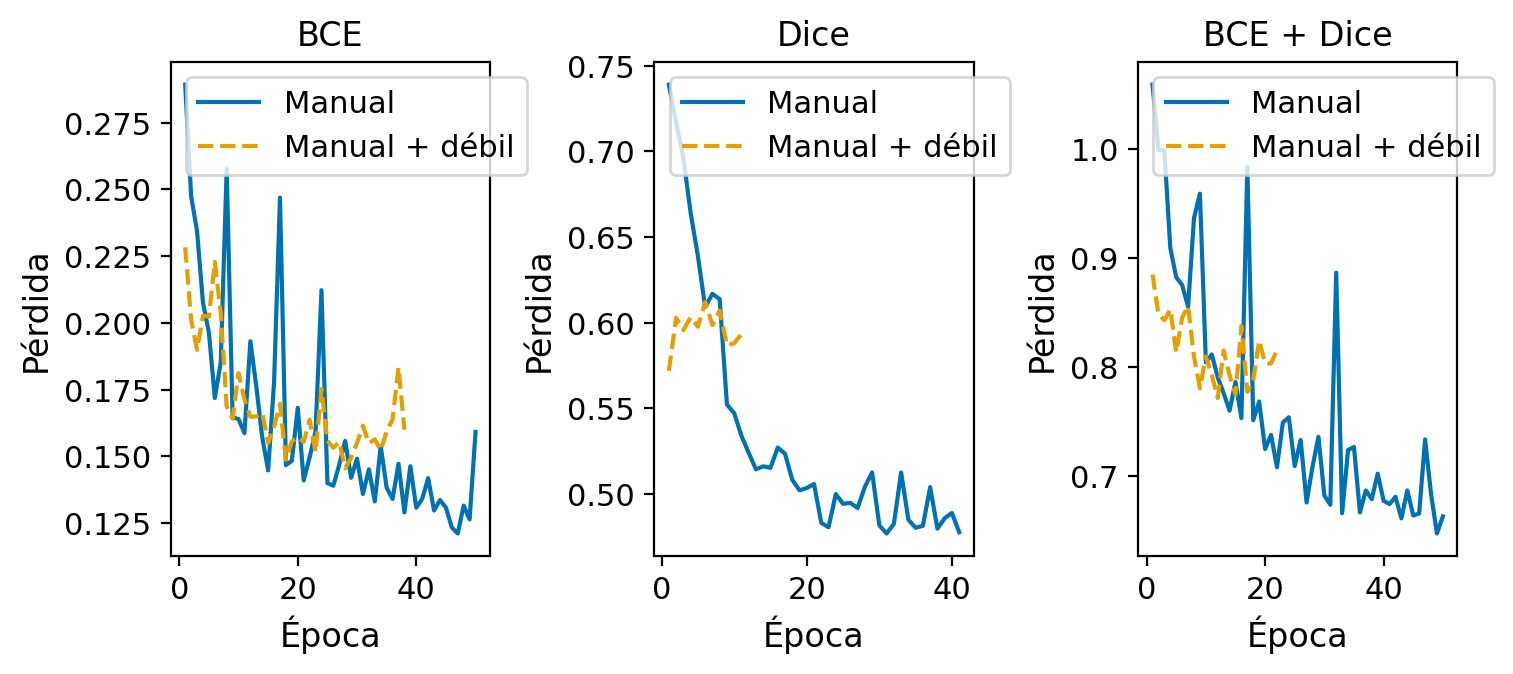
\includegraphics[width=0.96\linewidth]{figures/flood_0.png}\caption{Validación manual por pérdida y fuente de supervisión.}\end{figure}
\begin{figure}[H]\centering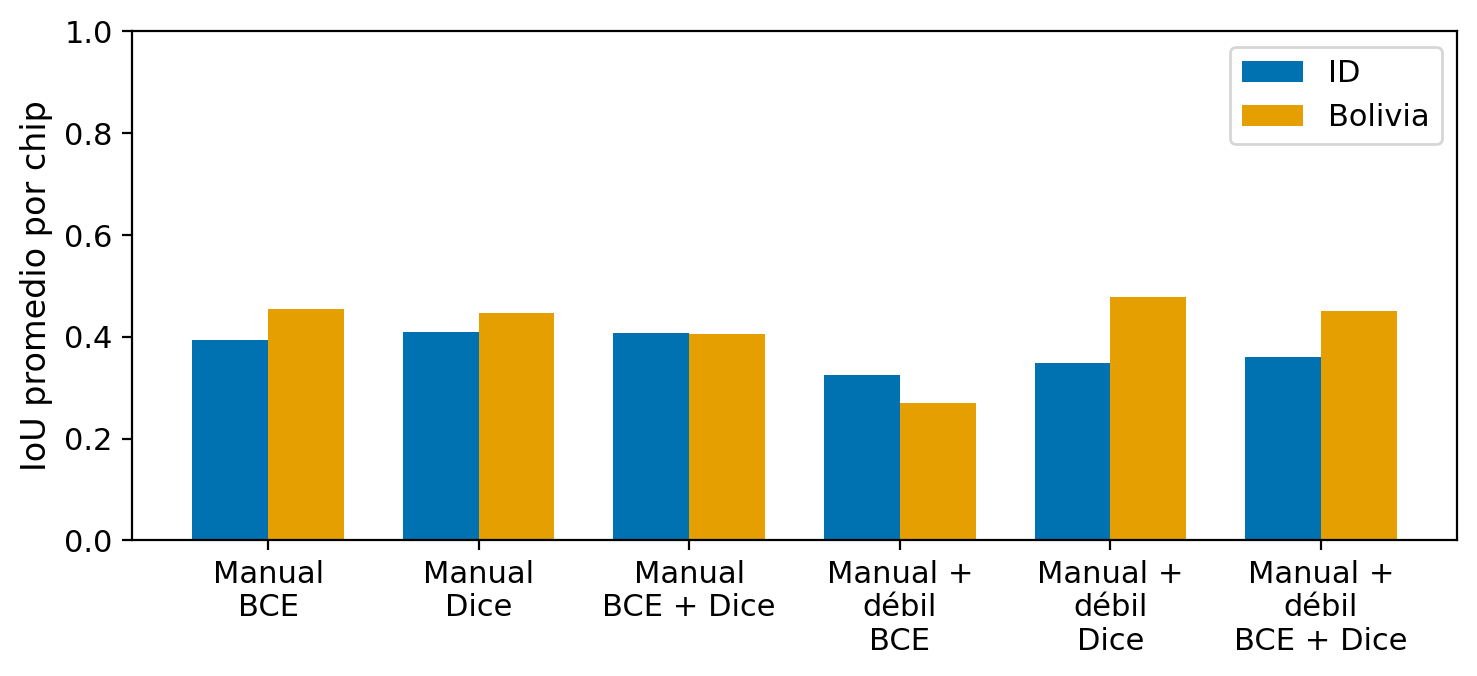
\includegraphics[width=0.96\linewidth]{figures/flood_1.png}\caption{Comparación de las seis configuraciones en ID y Bolivia.}\end{figure}
\begin{figure}[H]\centering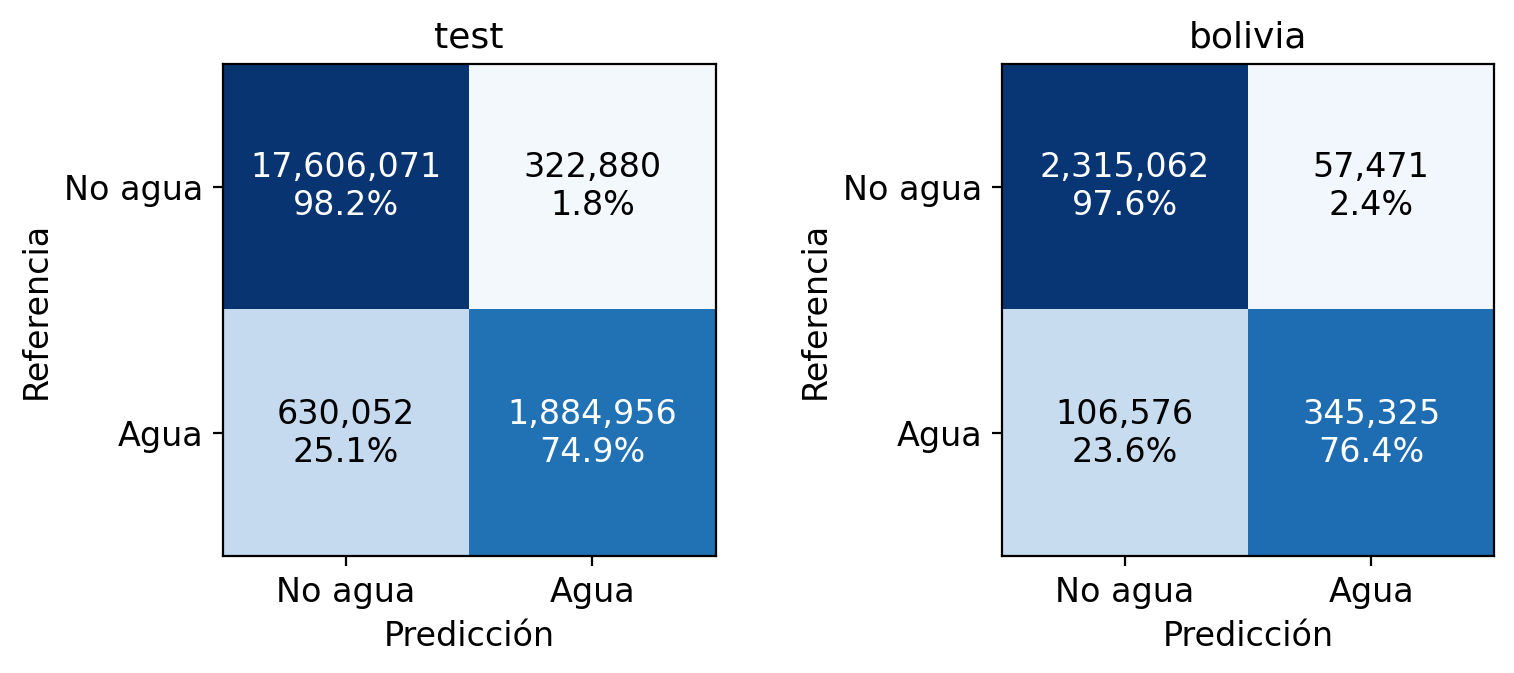
\includegraphics[width=0.96\linewidth]{figures/flood_2.png}\caption{Baseline gold+BCE: conteos y porcentajes normalizados por clase real.}\end{figure}

\section{Errores SAR y generalización}
\subsection{Tres patrones observados en el baseline}
\paragraph{Falsos positivos de baja retrodispersión.}
En \texttt{Pakistan\_70625}, las manchas oscuras a la izquierda y arriba reciben alta
probabilidad aunque la referencia solo marca cauces estrechos. Hay 28\,116 FP y
3\,330 FN; la IoU es 0.0408. La mediana VV/VH de los FP es $-17.84/-25.82$ dB,
frente a $-9.07/-17.93$ dB en verdaderos negativos. La señal de los FP se parece a
la del agua correctamente detectada ($-18.01/-26.03$ dB). Esto evidencia ambigüedad
radiométrica en el chip. Superficies lisas o sombra de radar son explicaciones físicas
posibles~\cite{sarhandbook}, pero aquí no se demuestra cuál opera: faltan cobertura,
topografía y una referencia óptica independiente.

\paragraph{Omisión de agua con respuesta más alta.}
En \texttt{Pakistan\_849790}, la referencia marca gran parte del chip como agua,
mientras la predicción retiene principalmente las regiones oscuras. Hay 138\,480 FN
y 793 FP, con recall 0.1945 e IoU 0.1936. La mediana VV/VH de los FN es
$-9.09/-17.90$ dB; la de los TP, $-16.31/-24.80$ dB. El modelo omite agua etiquetada
cuya respuesta difiere de la del agua oscura. Vegetación inundada, rugosidad o doble rebote
pueden cambiar la respuesta SAR~\cite{sarhandbook}; no se identifican esos mecanismos
únicamente por VV/VH. También deben considerarse incertidumbre de anotación y adquisición.

\paragraph{Fragmentación y bordes de cauces estrechos.}
En \texttt{Bolivia\_379434}, el cauce sinuoso derecho presenta bandas próximas de FP y FN
y tramos discontinuos. Se omite además una mancha central de agua. El chip tiene 5\,588 FP,
6\,528 FN e IoU 0.2602. El 81.25\% de los 12\,116 errores cae en una banda de borde
definida por dilatación/erosión binaria de la referencia con tres iteraciones.
Esa concentración apoya un problema de detalle espacial; no demuestra un desplazamiento
global de registro. Las transformaciones imagen/máscara fueron verificadas y se exportó
sin remuestrear. Resolución efectiva, contexto del encoder y definición del límite son
hipótesis adicionales, que deberían contrastarse con recortes y referencias independientes.

Los tres casos fueron inspeccionados técnicamente y registrados en
\texttt{qualitative\_cases.csv}; requieren revisión editorial del grupo.
Los patrones pueden coexistir y sus conteos no representan categorías causales mutuamente
excluyentes. No se afirma que una imagen oscura sea necesariamente agua o sombra.
\begin{figure}[H]\centering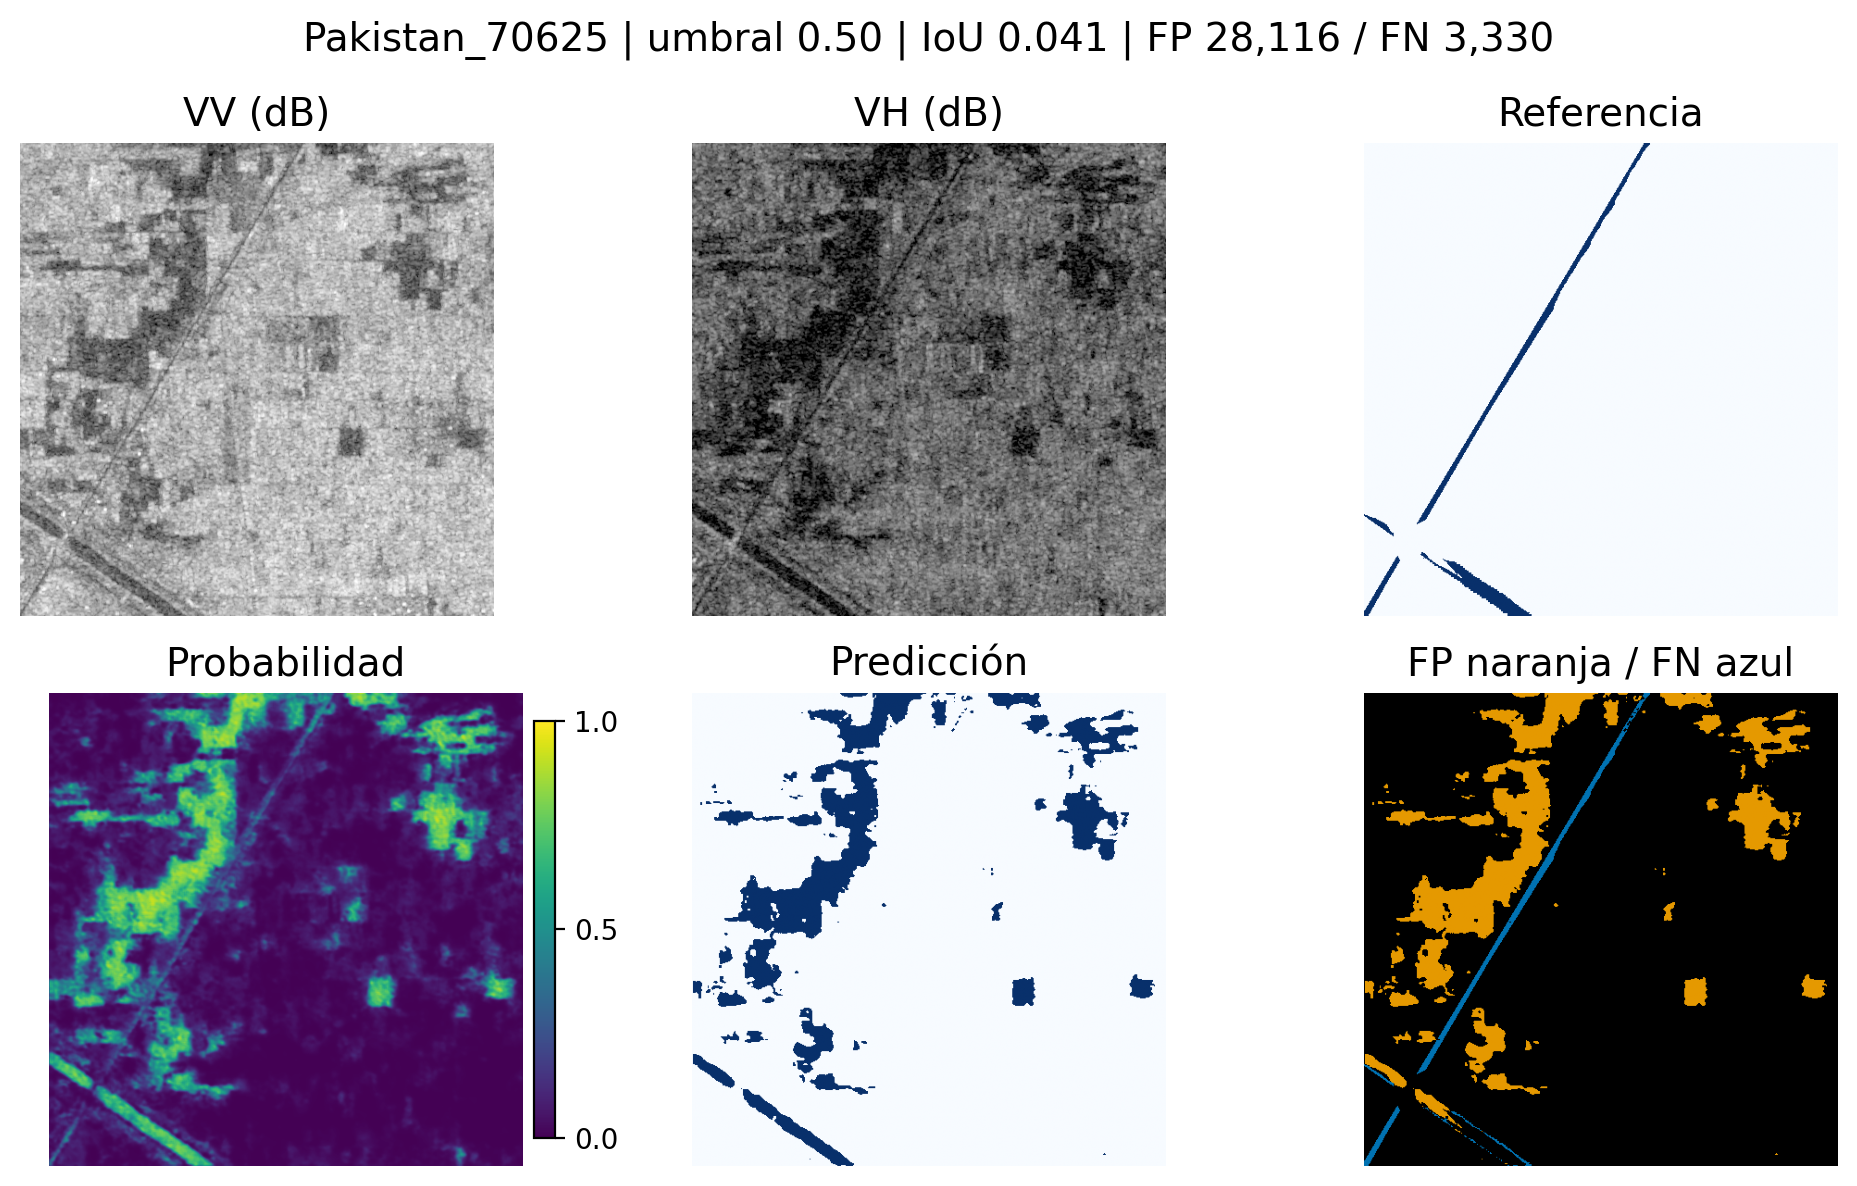
\includegraphics[width=0.96\linewidth]{figures/flood_3.png}\caption{Pakistan\_70625 (test): Se predicen manchas extensas en zonas oscuras sin agua en la referencia; el cauce diagonal fino queda parcialmente omitido.}\end{figure}
\begin{figure}[H]\centering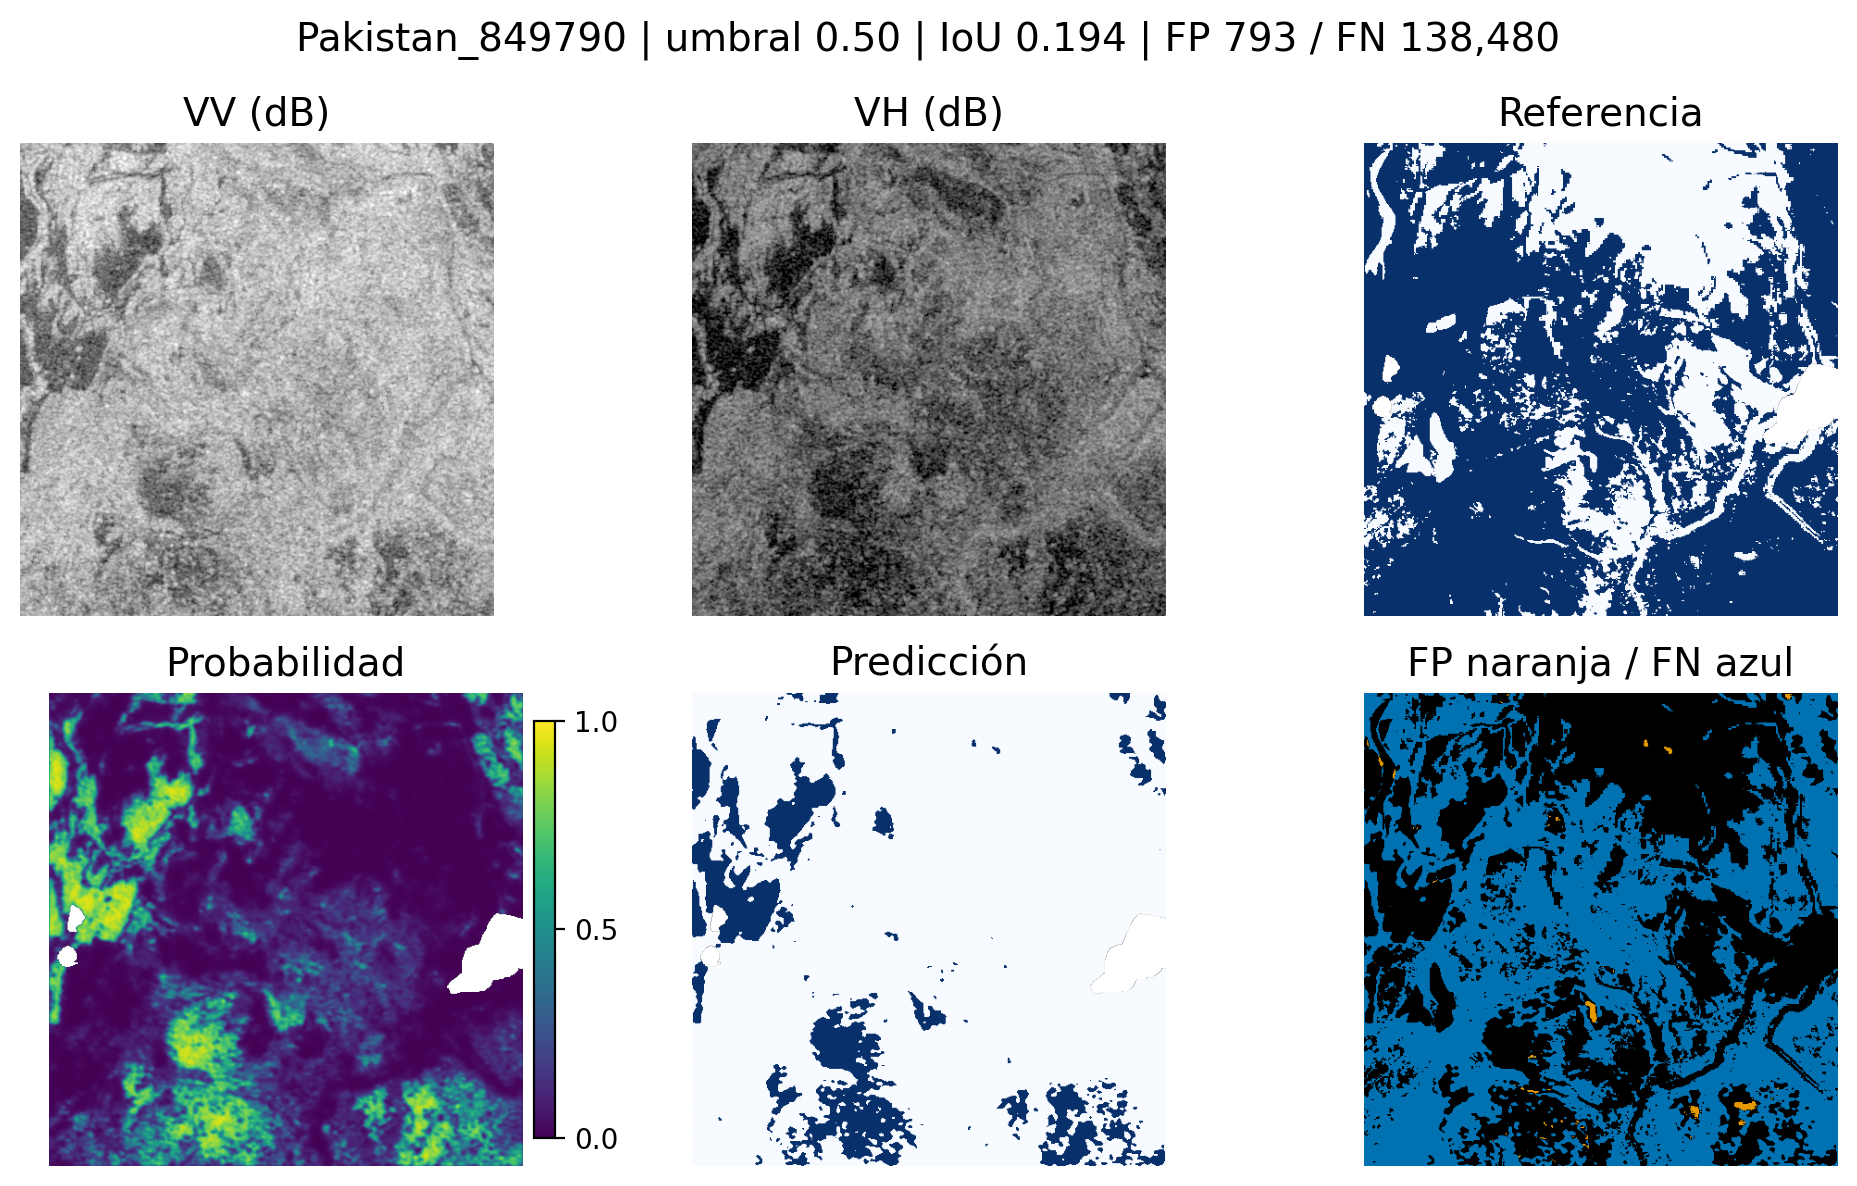
\includegraphics[width=0.96\linewidth]{figures/flood_4.png}\caption{Pakistan\_849790 (test): La referencia cubre gran parte del chip pero la predicción retiene pocas zonas oscuras; predominan falsos negativos en superficies de respuesta más alta.}\end{figure}
\begin{figure}[H]\centering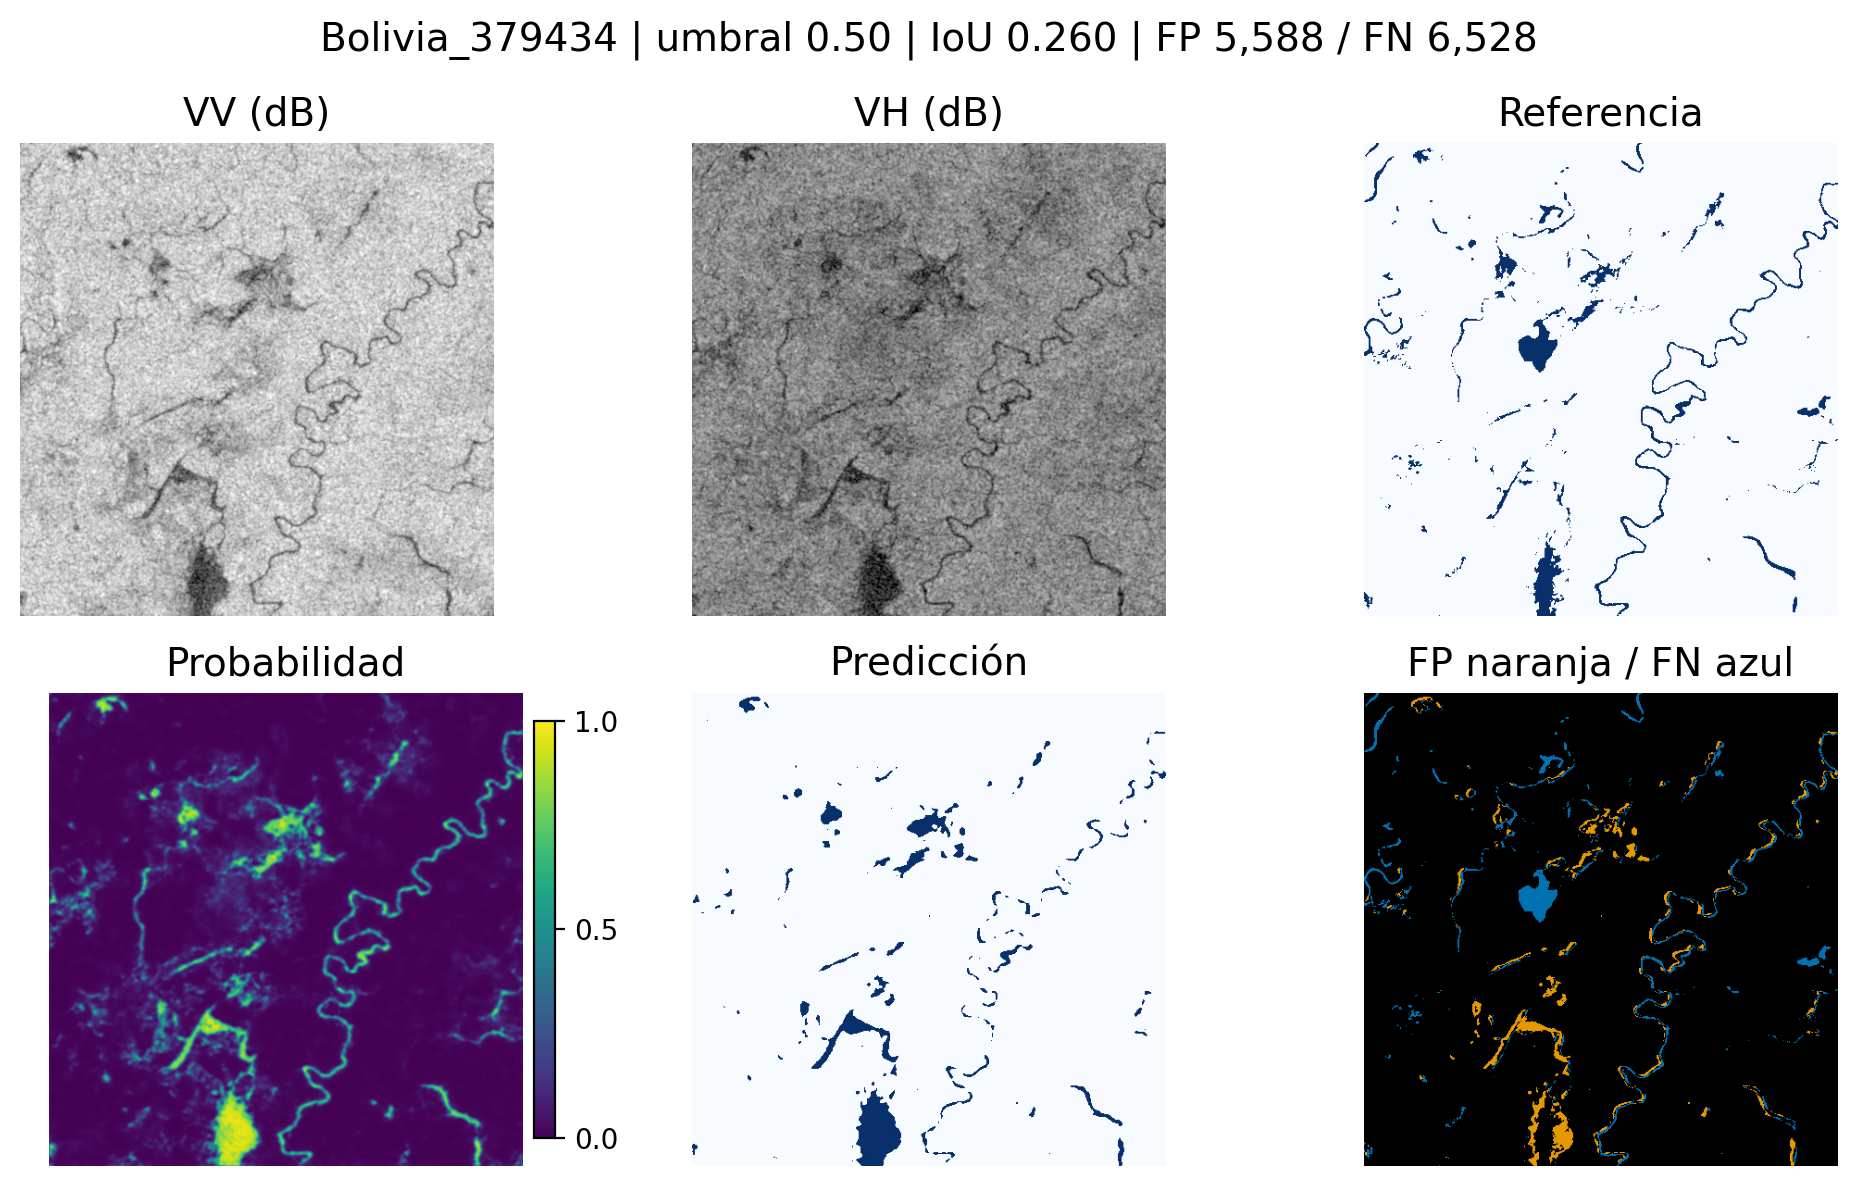
\includegraphics[width=0.96\linewidth]{figures/flood_5.png}\caption{Bolivia\_379434 (bolivia): En el cauce sinuoso derecho aparecen bandas cercanas de FP y FN y tramos fragmentados; también se omite una mancha central de agua.}\end{figure}

\subsection{Dos hipótesis de generalización}
\paragraph{H1: cambia la distribución de apariencia y prevalencia del agua.}
Bolivia tiene 16.00\% de agua válida, frente a 12.30\% en prueba ID y 9.55\% en entrenamiento.
Diferentes proporciones de agua abierta, canales y agua de respuesta alta pueden cambiar
precisión, recall e IoU. Los ejemplos muestran que la respuesta del agua no es uniforme.
Un test de esta hipótesis separaría resultados por cobertura, amplitud VV/VH y tamaño de
regiones, usando anotaciones independientes. La prevalencia medida es evidencia descriptiva;
no demuestra por sí sola una causa de la brecha.

\paragraph{H2: cambian adquisición y sesgo de etiquetas débiles.}
Los metadatos oficiales ubican Bolivia en órbita descendente relativa 156, el 15 de febrero
de 2018. También hay adquisiciones descendentes en entrenamiento, por ejemplo India,
Pakistán y Paraguay; por ello, la dirección descendente no explica por sí sola una diferencia externa.
El número de órbita relativo y la geometría local podrían modificar la señal, pero no
se dispone del ángulo de incidencia por chip. Además, las etiquetas débiles derivadas
de umbralización SAR pueden reforzar la asociación entre agua y baja retrodispersión.
Para contrastarlo se necesitarían geometría/incidencia, cobertura y una comparación con
presupuesto igual de pasos, múltiples semillas y máscaras manuales adicionales.
Bolivia representa un evento externo pequeño; una brecha positiva o negativa no aísla
un efecto geográfico y no permite generalizar a todos los países.

El baseline cualitativo es \texttt{gold\_bce}, fijado antes de observar prueba o Bolivia.
Se inspeccionan candidatos de menor IoU y, cuando hace falta, casos con falsos positivos,
falsos negativos o límites estrechos. Esta selección es intencional y no estima la
frecuencia de causas en la población. Cada panel conserva el mismo rango VV/VH
($-30$ a 0 dB), probabilidad de 0 a 1 y el umbral fijo. Los mapas GeoTIFF exportados
mantienen CRS y transformación original, con nodata -1.

\section{Limitaciones, conclusiones y reproducción}
La supervisión débil mejora la IoU principal en 0 de tres pérdidas en ID y en 2 de tres en Bolivia. La matriz permite observar sensibilidad a la pérdida y a la fuente de etiquetas, sin demostrar una mejora universal ni aislar el efecto de las etiquetas del número de actualizaciones. Los casos cualitativos muestran ambigüedad radiométrica, omisión de agua de respuesta alta y errores de detalle espacial. La evaluación externa debe conservar la agregación y el signo real de la brecha.


Una única semilla y quince chips externos no permiten afirmar significancia estadística
ni estimar incertidumbre entre eventos independientes. Los chips pueden compartir evento
y vecindad espacial; respetar los CSV oficiales no garantiza independencia por evento.
La validación manual contiene menos de cien chips y orienta tanto selección como parada.
La ponderación débil y el clipping son decisiones heurísticas fijadas previamente;
el experimento no busca umbrales, profundidades o pesos óptimos. Para aislar el efecto
de etiquetas débiles sería necesario igualar actualizaciones y repetir varias semillas.

La reproducción local usa \texttt{parcial/scripts/run\_flood.ps1}, con Docker Desktop,
WSL2 y GPU compatible con CUDA 12.8. El script construye el entorno, verifica la caché,
ejecuta controles, prueba corta, seis experimentos, notebook e informe. La opción
\texttt{-Resume} recupera el checkpoint de la última época terminada y rechaza cambios
de firma de datos o configuración. Si aparece el entrenamiento del ejercicio 3, preserva
el estado de inundaciones, espera y retoma. No detiene procesos ajenos. Las salidas quedan
en \texttt{E:/Kaggle/exam-output-flood}; datos y resultados no se incluyen en Git.

El entorno usa Python 3.12, PyTorch 2.10.0, CUDA 12.8 y Rasterio 1.4.3.
Los manifiestos, configuración congelada, hashes de fuente, historial, checkpoints,
conteos por chip y metadatos de ejecución permiten rastrear cada cifra. Las pruebas cortas
se guardan en otra carpeta y quedan excluidas del informe científico. El repositorio
configurado es \url{https://github.com/miguelsff/maestria-ia-uni-ciclo-2-redes-neuronales};
las modificaciones locales requieren publicarse para que otra persona pueda reproducir
esta revisión desde GitHub. La autoría real del grupo está pendiente de completar.
\bibliographystyle{plain}
\bibliography{flood_references}
\end{document}
